\section{Test}
The aim of the project is to create a good base on which multiplayer games can easily be created. It is therefore desirable that the server is stable and able to handle a decent number of games at the same time without significant response time. More specifically we want a single server to be able to host as many games as possible without surpassing an average response time of 0.5 seconds. Additionally we want to locate possible bottlenecks in the code, by recording the run time of each API call. This can be tested using a black-box testing.

The Python scripts used to test the server can be found in the folder named Test with the rest of the source code.\fixme{ret i forhold til hvor det ligger}

\subsection{Test Setup}
\label{sec:testSetup}
The test is done by simulating users through Python scripts: One for simulating a number of active games with the purpose of creating some artificial server load, and one for making single API calls and collecting data.

The first script creates server load by spawning a thread per desired game. Each thread creates a game, makes relevant API calls for the duration of the test, and finally it deletes the game. Each thread simulates very busy games with 2 API calls per second. 

The other script makes a single API call a number\fxfatal{what number?} of times, collects the run time for each call and finally calculates the mean and standard deviation. Because the goal is to stay on a run time under 0.5 seconds, the number of calls taking more than this is also recorded.

Each script is run on seperate computers, to be sure the extra processing power needed to handle the game threats does not influence the test results. 

%The following API calls are used in the test:
%\begin{itemize}
%\item Login
%\item Create game
%\item Delete game
%\item Join game
%\item Leave game
%\item Change location
%\item Invite player
%\item List public games
%\item List joined games
%\item Get game info
%\item Shoot
%\end{itemize}

\subsection{Analysis of Test Results}
The tests have now been concluded and the results can be analyzed. show the results and the raw data is available along with the source code in the Test folder.\\

After running the script the first time, the script failed, and we were given a timeout exception. We then modified the test to record these timeouts and continue the test, but the exact source of the exception was not located. The script was run 1000 times with each API call, and the calls that timed out were not included in the final test results.\\

% % % tables
\Cref{tab:unloadgraph} shows the mean of the response time for each API call. As can be seen the mean is mostly the same for all API calls except for the Get joined games call. We suspect this is because of the way data is stored in the database. This response time could be lessened by routinely deleting old games from the table containing created games. This is currently not done but the overall the mean is below the threshold of 0.5 seconds.\\

The table also shows the number of calls exceeding the maximum allowed response time of 0.5 seconds. Also here Get joined games has the highest response time, but for all the API calls only 1-3 out of the thousand calls exceeded the limit. Looking at the raw data, shows that these calls sometimes took 4-6 seconds, and in rare cases completely timed out. It is difficult to say where exactly the problem arises, but due to the low amount of slow or timed out calls, we argue that these results are satisfactory in regards to the timeout threshold of 0.5 seconds.\\

\Cref{tab:loadgraph} shows the results of the test when the server was handling 100 busy games. By trial and error this was found to be the maximum amount of games the server could consistently handle without timing out completely.\\

As can be seen, the mean response for each API call has increased from the response times in \Cref{tab:unloadgraph}. This is mainly because of the increased load on the server from the 100 busy games running concurrently. \Cref{tab:loadgraph} also shows the Get joined games API call as the API call with the largest response time. This confirms that it was not just by chance \Cref{tab:unloadgraph} showed the same.\\

Not unexpectedly, it can be seen that there are more API calls which exceed the timeout threshold of 0.5 seconds. An interesting observation, however, is the fact that less API calls timed out, as one would expect the case to be the opposite with the increased load on the server. This could indicate that there is an error somewhere in the server or the network connection that sometimes encountered.\\

% % % graph
Looking on the graph on \Cref{fig:loadgraph} a general pattern can be seen. For the first approximately 90 runs of the 11 API calls the response time is reasonably low. Given the heavy load on the server many are still over the threshold of 0.5 seconds, but that is to be expected, and it is positive that the response time is relatively stable until then. After that several big spikes can be observed, followed closely by period of very good response time. This is especially noticable around run 160 and 710. A couple of things could be the cause of this, and most likely it shows the server getting overloaded and dropping some connections, followed by good performance until the connections are reestablished.\\

A similar graph for the results of the test without load does not show anything noteworthy - most calls are very fast, and there are a few spikes, but there is no observable pattern. Generally, we would expect better results with fewer active games, but it is difficult to predict how many it would realistically run, as it depends a lot on the activity of each game.\\\\

% % % sources of error
We discovered some issues with the test, which could have affected the results.\\
First of all, both the server, the spammer and the computer measuring the response time of the server were connected through a local mobile hotspot. This network was not the most stable, and it could therefore have affected the response times in a way that would not happen if they had been connected to a more stable network.\\
Another issue is that the test was run through an IDE. This could have affected the response times because the IDE may have caused some performance overhead. This could be remedied by running the test outside of the IDE.\\
The computers used for testing, except for the server, were in use while the tests were running. This could possible have affected the response times as well. A remedy for this could be to simply have dedicated computers running nothing except only what they are supposed to.\\
Lastly, there was only one computer attempting to overload the server at one time. This means that if that computer was affected in a way which affected its performance I/O wise, all of the overload on the server is reduced. This could also have affected the test results since the server would not have been continually overloaded, as was intended. It could be remedied by having multiple computers attempting to overload the server at the same time, since it is unlikely all of them would have performance problems at the same time.

%In table \cref{tab:testRes} the results from the test are shown\fixme{Just latency test?}. Each test was perfomed with half a second interval.

\begin{figure}[H]
  \centering
  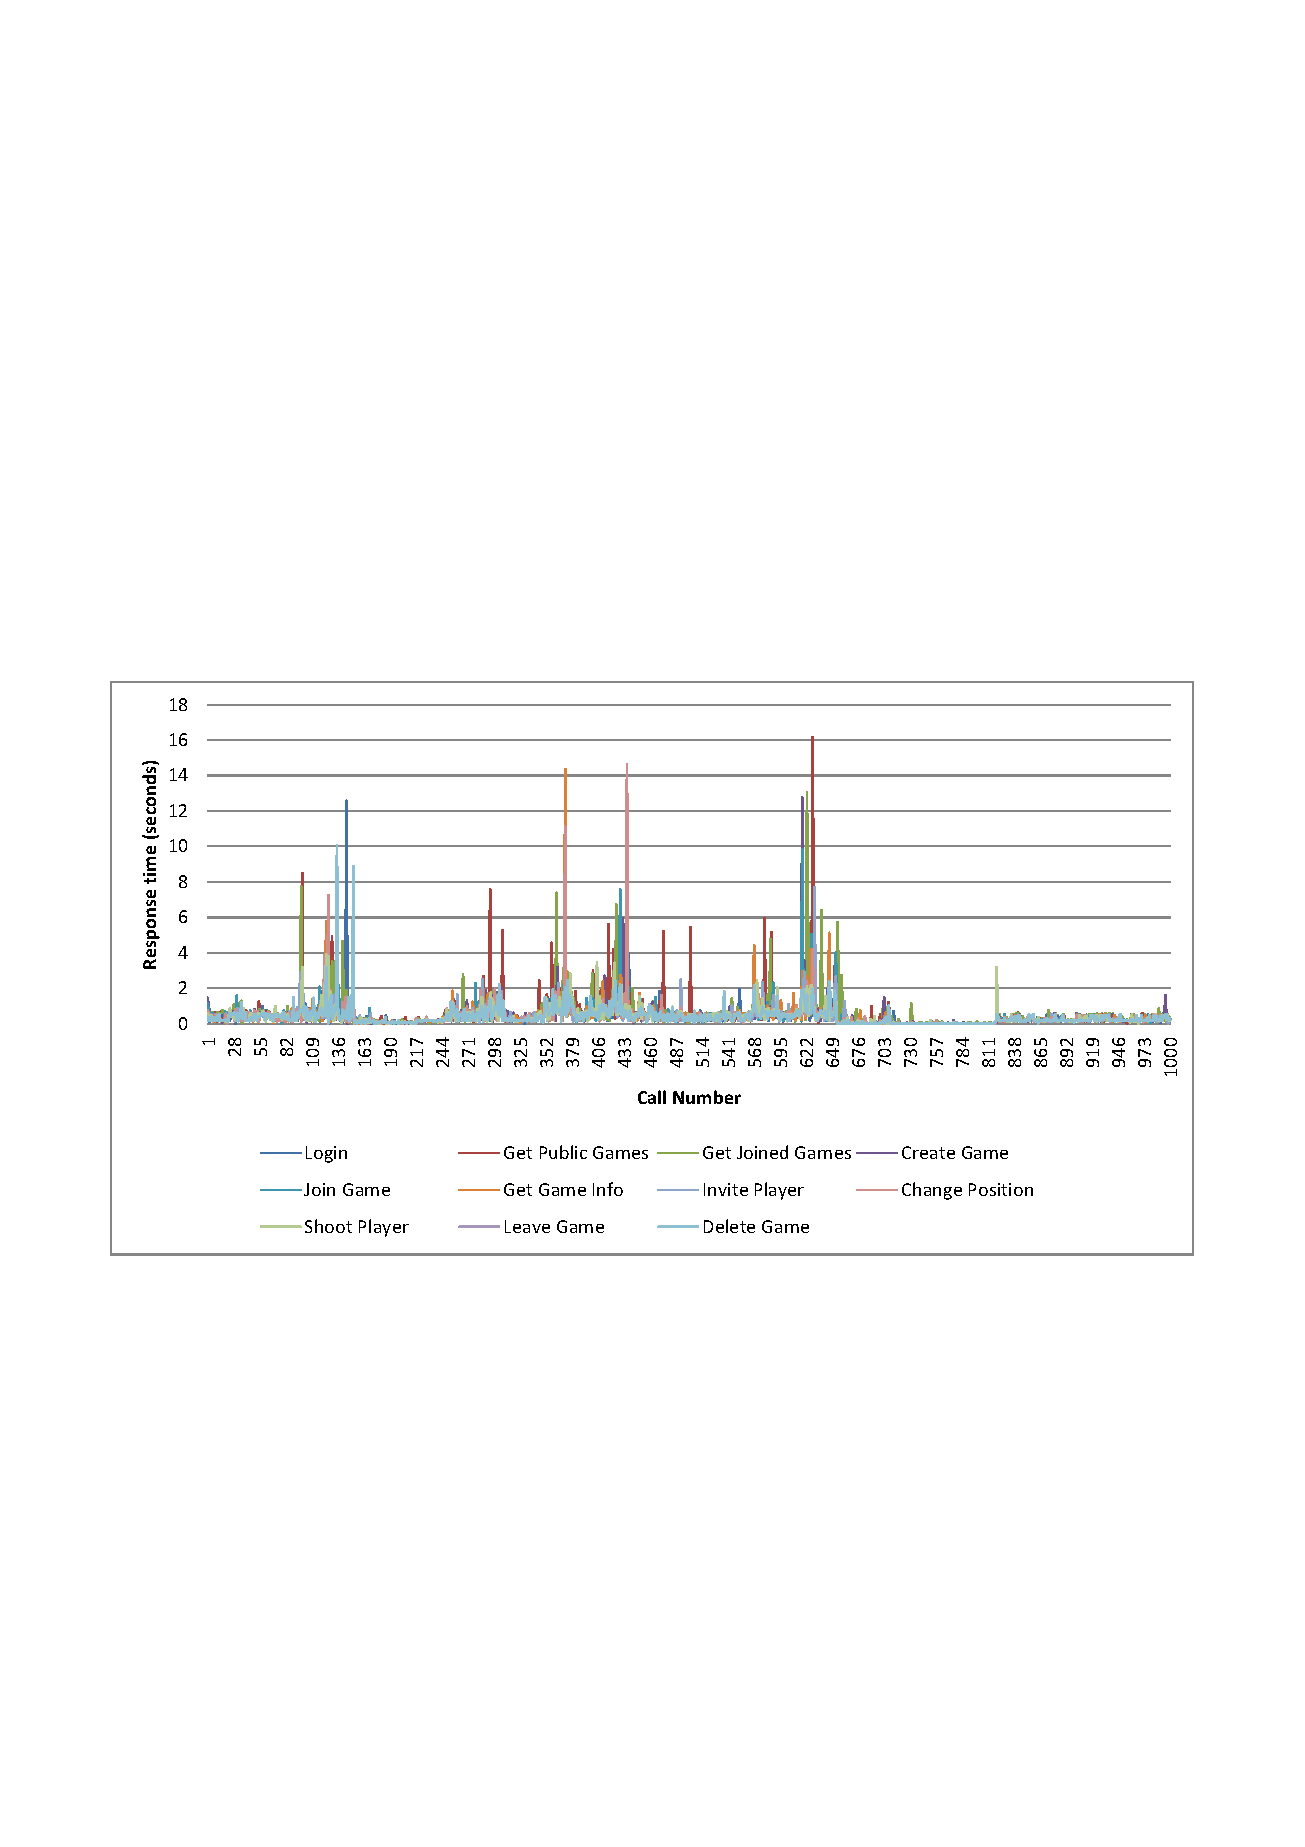
\includegraphics[width=\textwidth, clip=true, trim=0 22em 0 22em]{billeder/loadgraph.pdf}  
  \caption{Graph showing the response time of each API call.}
  \label{fig:loadgraph}
\end{figure}

\renewcommand{\arraystretch}{1.2}
\begin{table}
\caption{Test with no load}
\label{tab:unloadgraph}
\centering
\begin{tabular}{|l|>{\raggedleft\arraybackslash}p{5em}|>{\raggedleft\arraybackslash}p{5em}|>{\raggedleft\arraybackslash}p{5em}|>{\raggedleft\arraybackslash}p{5em}|}
	\hline  & \multicolumn{1}{p{5em}|}{Mean of response time (sec)} & \multicolumn{1}{p{5em}|}{Number over limit} & \multicolumn{1}{p{5em}|}{Number timed out} \\ 
	\hline Login  & 0.0135 & 3 & 0 \\ 
	\hline Get public games  & 0.0118 & 2 & 0 \\ 
	\hline Get joined games  & 0.0565 & 10 & 1 \\ 
	\hline Create game  & 0.0131 & 1 & 0 \\ 
	\hline Join game  & 0.0118 & 2 & 0 \\ 
	\hline Get game info  & 0.0114 & 2 & 0 \\ 
	\hline Invite player  & 0.0100 & 1 & 0 \\ 
	\hline Change position  & 0.0097 & 0 & 1 \\ 
	\hline Shoot player  & 0.0168 & 3 & 0 \\ 
	\hline Leave game  & 0.0067 & 1 & 1 \\ 
	\hline Delete game  & 0.0102 & 0 & 0 \\ 
	\hline 
\end{tabular} 
\end{table}

\begin{table}
\caption{Test with load}
\label{tab:loadgraph}
\centering
\begin{tabular}{|l|>{\raggedleft\arraybackslash}p{5em}|>{\raggedleft\arraybackslash}p{5em}|>{\raggedleft\arraybackslash}p{5em}|>{\raggedleft\arraybackslash}p{5em}|}
	\hline  & \multicolumn{1}{p{5em}|}{Mean of response time(sec)} & \multicolumn{1}{p{5em}|}{Number over limit} & \multicolumn{1}{p{5em}|}{Number timed out} \\ 
	\hline Login  & 0.3676 & 262 & 1 \\ 
	\hline Get public games  & 0.4825 & 328 & 0 \\ 
	\hline Get joined games  & 0.4959 & 353 & 0 \\ 
	\hline Create game  & 0.4143 & 306 & 0 \\ 
	\hline Join game  & 0.4096 & 289 & 0 \\ 
	\hline Get game info  & 0.4051 & 279 & 0 \\ 
	\hline Invite player  & 0.3752 & 273 & 0 \\ 
	\hline Change position  & 0.4050 & 276 & 0 \\ 
	\hline Shoot  & 0.3806 & 259 & 0 \\ 
	\hline Leave game  & 0.3814 & 253 & 0 \\ 	
	\hline Delete game  & 0.3721 & 299 & 0 \\ 
	\hline 
\end{tabular} 
\end{table}
\renewcommand{\arraystretch}{1}